% !Mode\dots ``TeX:UTF-8''
% !TEX root = ../root.tex
\section{Algorithm for determining the online observability}
\label{sec:deter}
The essence of determining the online observability of \BCN\ is to determine the $k$-step determinability of every non-empty $\Ded(\Delta_N,\varepsilon, \mathsf{o}^{j}(0))$. 

\subsection{Input-labelled graph}
We define a directed graph for \BCN\ named input-labelled graph. Based on the input-labelled graph and the way to construct it, we can propose determination algorithm for the online observability.

\begin{definition}[Input-labelled Graph]
Let $\mathcal{V}$, $\mathcal{E}$ and $\mathcal{L}$ be the vertex set, the edge set and the labelling function of an input-labelled graph $\mathcal{G}=(\mathcal{V}, \mathcal{E}, \mathcal{L})$. $\mathcal{G}$ is called the input-labelled graph of the \BCN\, if 
\begin{itemize}
\item  $\mathcal{V}=\{\mathsf{S}\in\bigcup_{j=0}^{(2^m -1)} 2^{\Ded(\Delta_N,\varepsilon,\delta^j_{2^m} )}|$ there exists a $k\ge0$ such that $\mathsf{S}$ is $k$-step determinable$\}$;
\item  $\mathcal{E}=\{(\mathsf{S}_1,\mathsf{S}_2)\in \mathcal{V}\times \mathcal{V}|$ there is an input $\mathsf{i} \in \Delta_M$ such that \[|\Ded\left(\mathsf{S}_1,\mathsf{i},\varepsilon\right)|=|\mathsf{S}_1|,\] and for every $\Ded(\mathsf{S}_1,\mathsf{i},\mathsf{o}^{j})\neq \emptyset$ $\Ded(\mathsf{S}_1,\mathsf{i},\mathsf{o}^{j})\in \mathcal{V}$, \[\mathsf{S}_2\in\{\Ded(\mathsf{S}_1,\mathsf{i},\mathsf{o})| \Ded(\mathsf{S}_1,\mathsf{i},\mathsf{o})\neq \emptyset, \mathsf{o}\in \Delta_Q\}\};\]
\item  $\mathcal{L}=\{\mathcal{E}\mapsto 2^{\Delta_M}|(\mathsf{S}_1,\mathsf{S}_2)\mapsto\{\mathsf{i}\in \Delta_M|$\[|\Ded\left(\mathsf{S}_1,\mathsf{i},\varepsilon\right)|=|\mathsf{S}_1|,\] and for every $\Ded(\mathsf{S}_1,\mathsf{i},\mathsf{o}^{j})\neq \emptyset$, $\Ded(\mathsf{S}_1,\mathsf{i},\mathsf{o}^{j})\in \mathcal{V}$, \[\mathsf{S}_2\in\{\Ded(\mathsf{S}_1,\mathsf{i},\mathsf{o})| \Ded(\mathsf{S}_1,\mathsf{i},\mathsf{o})\neq \emptyset, \mathsf{o}\in \Delta_Q\}\}\}.\]
 \end{itemize}
\end{definition}

\begin{figure}[thpb]
      \centering
      \framebox{\parbox{3in}{
		\centerline{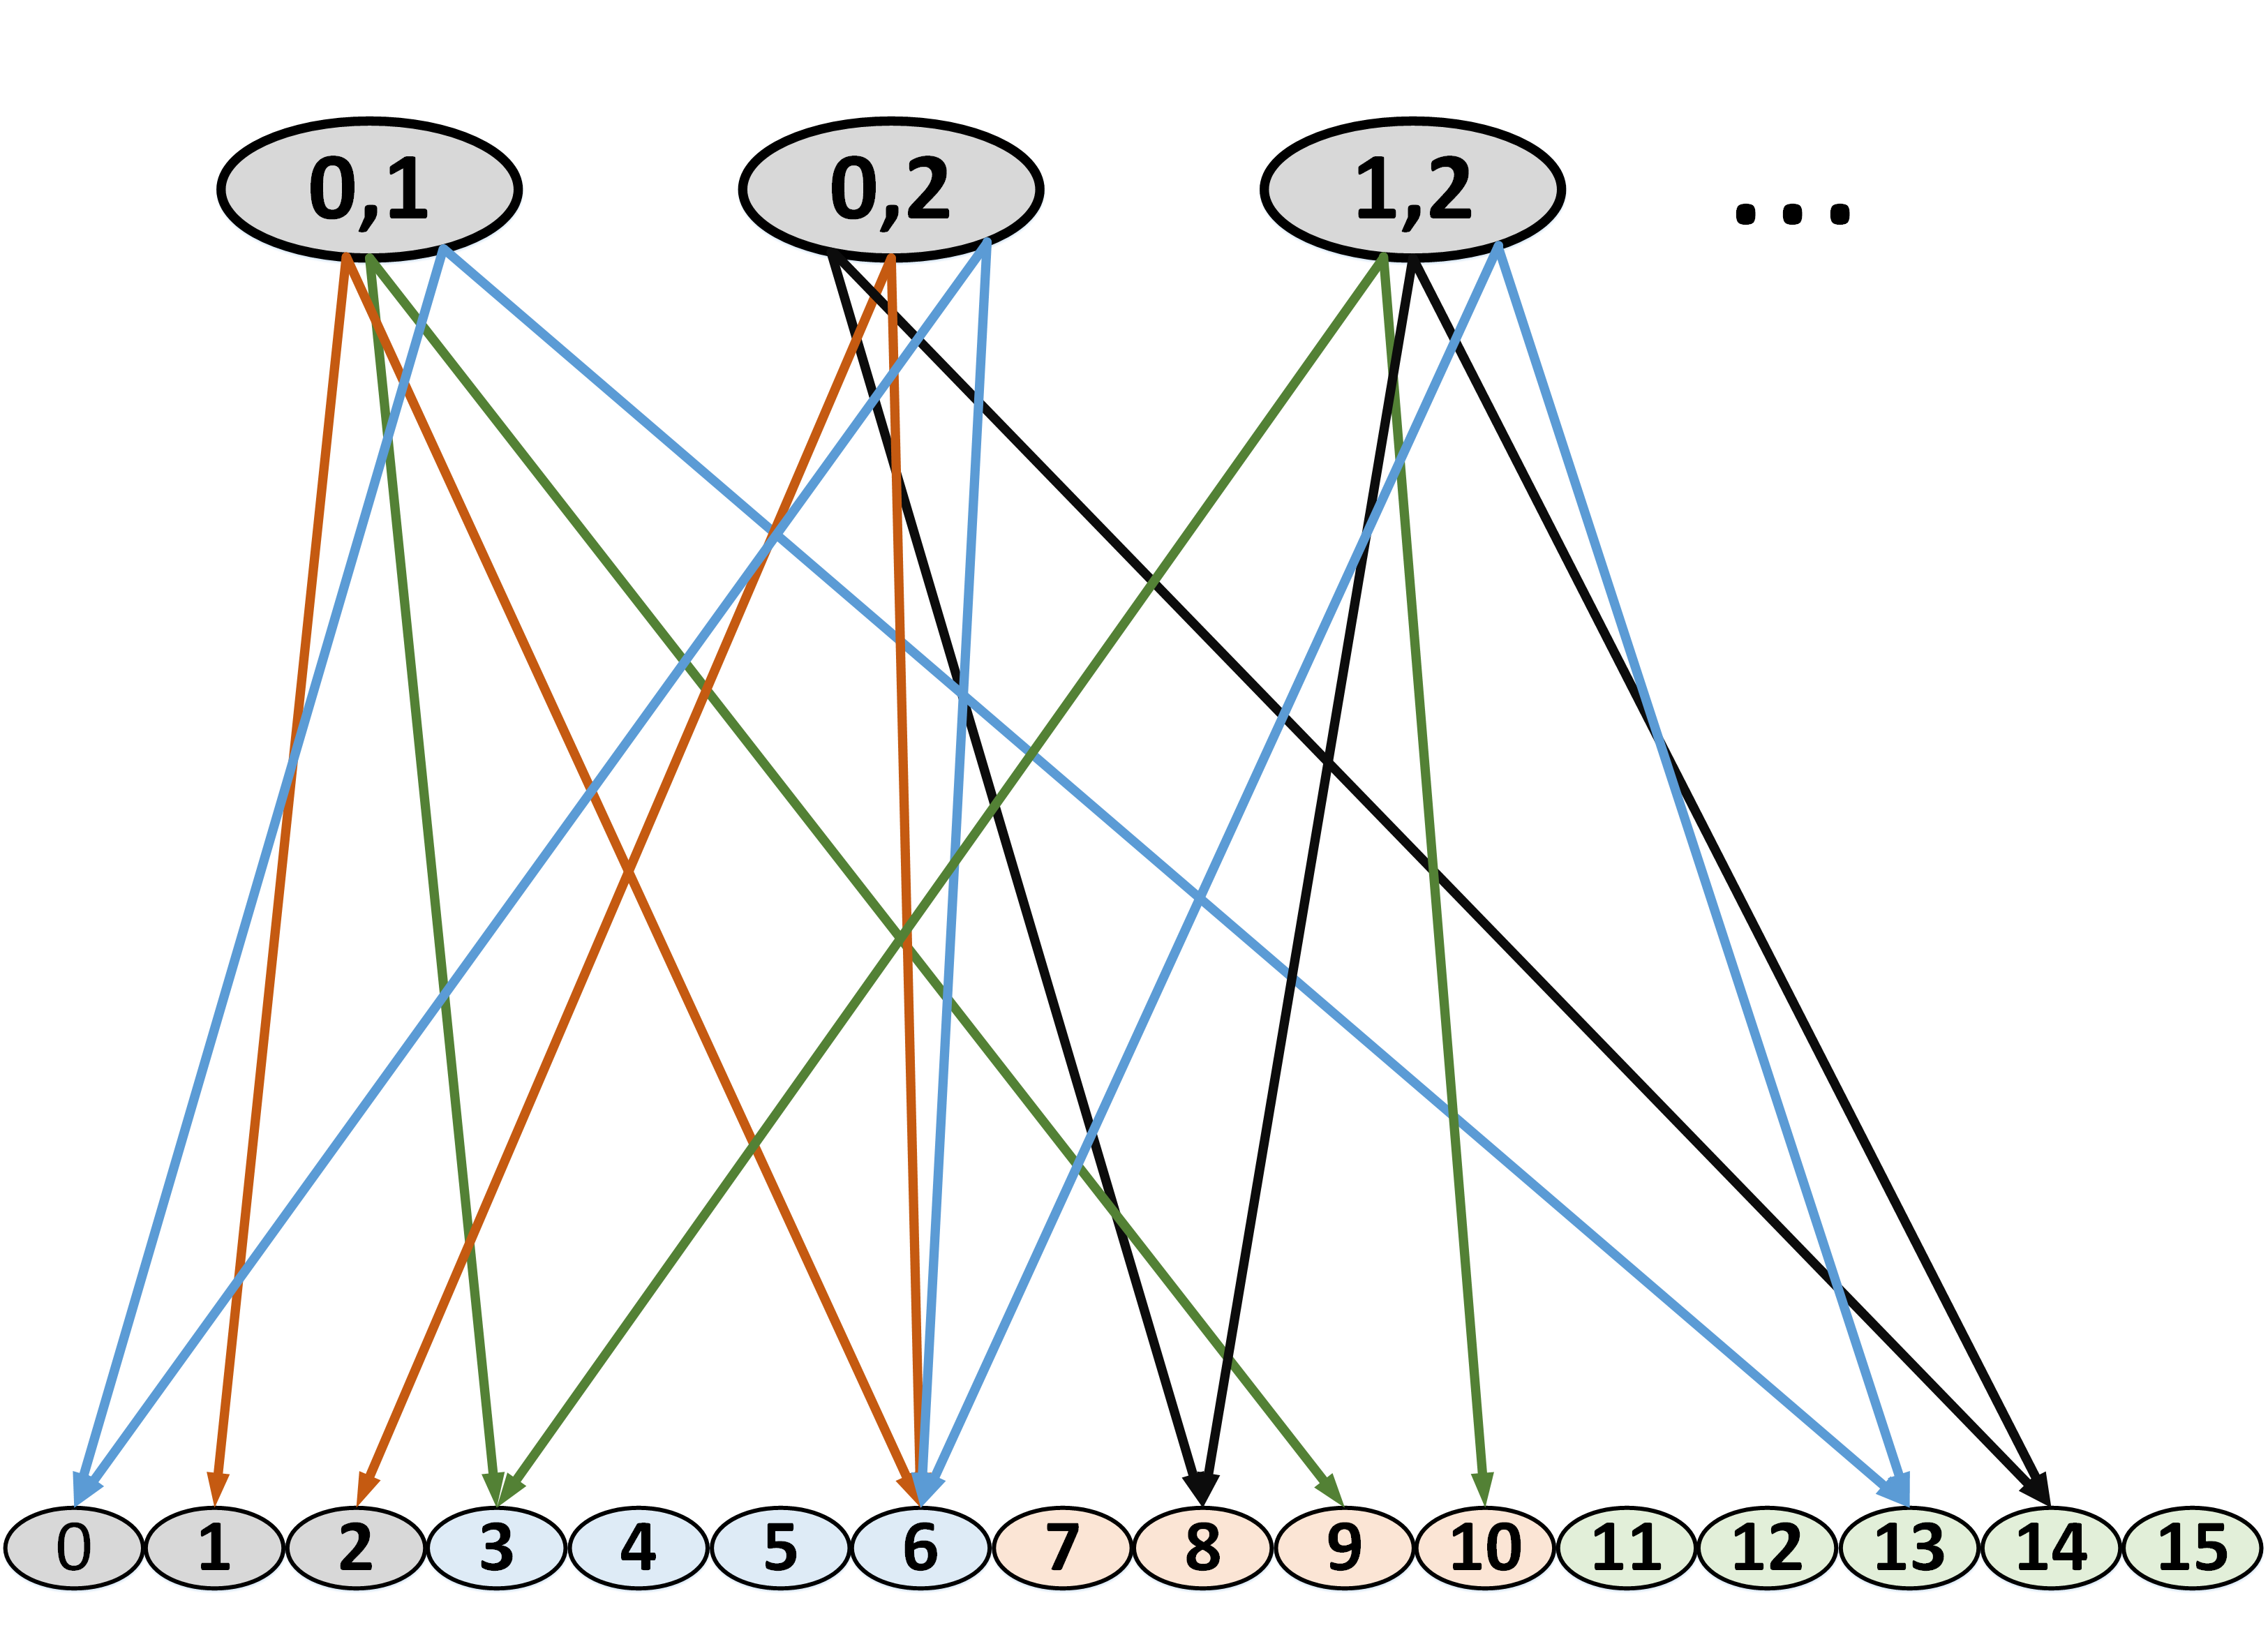
\includegraphics[scale=0.090]{figures/Fig4.png}}
	}}
      
      \caption{Part of the input-labelled graph, where the green, black, orange, blue edges are labelled with $\{\delta_4^0\}$, $\{\delta_4^1\}$, $\{\delta_4^2\}$ and $\{\delta_4^3\}$ respectively.}
      \label{fig:4}
\end{figure}

Intuitively, the vertex of the input-labelled graph represents the set of states $\mathsf{S}$ of the \BCN\ which satisfy $k$-step determinability for some $k>0$, and every state in $\mathsf{S}$ with identical corresponding output. Thus determine the $k$-step determinability of every non-empty $\Ded(\Delta_N,\varepsilon, \mathsf{o}^{j}(0))$ and then determine the online observability by checking the input-labelled graph.

From the {\em Lemma \ref{lemm:2}}, we have that if for the set of states $\mathsf{S}^1$ there does not exist any $k^{1}\ge 0$ such that $\mathsf{S}^{1}$ is $k^{1}$-step determinable, and $\mathsf{S}^{1}\subseteq \mathsf{S}^{2}$. Then there does not exist any $k^{2}\ge 0$ that make $\mathsf{S}^{2}$ $k^{2}$-step determinable. Therefore, in the process of building input-labelled graph for a \BCN\ we build the vertexes with fewer states at first, and then build the vertexes with more states.
\begin{itemize}
\item  Because, once we can find vertex $\mathsf{S}^x$, such that there does not exist any $k^{x}\ge0$ makes $\mathsf{S}^{x}$ $k^{x}$-step determinable. And we know that there exists $\mathsf{o}^{j}\in \Delta_Q$ such that $\mathsf{S}^{x}\subseteq \Ded\left(\Delta_N,\varepsilon, \mathsf{o}^{j}\right)$. We have for $\Ded\left(\Delta_N,\varepsilon, \mathsf{o}^{j}\right)$, there does not exist any $k^{j}\ge 0$ that makes  $\Ded\left(\Delta_N,\varepsilon, \mathsf{o}^{j}\right)$ $k^{j}$-step determinable either, and then the \BCN\ is not online observable.
\item And as we determine the $k$-step determinability of every $\Ded(\mathsf{S}_x,\mathsf{i}^{x},\mathsf{o}^{j})$, we can determine the $k$-step determinability of $\mathsf{S}_x$ easily.
\item  Finally, as the $k$-step determinability of the subsets of $\mathsf{S}_x$ has been checked, it is convenient for us to find the $\mathsf{i}_x$ which makes $\mathsf{S}_x$ $k_x$-step determinable by the subsets of $\mathsf{S}_x$.
 \end{itemize}
 \subsection{Determination algorithm}
 We propose the {\bf Algorithm~\ref{alg:1}} to determine online observability based on input-labelled graph, and {\bf Algorithm~\ref{alg:1}} can also find all paths to determine $\mathsf{s}(0)$ if the \BCN\ is online observable.

\begin{itemize}
\item  Firstly, for every $n>0$ we try to build vertexes with $n$ states which with identical corresponding output. 
\item Secondly, if the vertexes can  be built, when $n>1$, we check the $k$-step determinability of the vertexes and build edges for them. And, if we can not build any edge for one vertex, we have the \BCN\ is not online observable.
\item Fianlly, if we can not build any vertex with $n$ states, then we have the $k$-step determinability of every non-empty $\Ded(\Delta_N,\varepsilon, \mathsf{o}^{j}(0))$ has been checked. Thus the \BCN\ is online observable.
 \end{itemize}

\begin{algorithm}[h]
\caption{Determination algorithm}
\begin{algorithmic}[1]
\REQUIRE 
The updating rules of \BCN
\ENSURE  
The directed graph of \BCN
\STATE Boolean value $Ob=$ true 
\STATE integer $i$ \
\STATE integer $j$ \
\STATE integer $n=1$
\STATE array $VertexArray[\ ]$
\STATE array $InputArray[\ ]$
\STATE {\sf buildvertex}($n$)
\STATE $n= n+1$
\STATE $VertexArray=${\sf buildvertex}($n$)
\WHILE {($VertexArray!=$Null)}
\FOR{($i=0$; $i<arraysize(VertexArray)$; $i++$)}
\IF{($p==2$)}
\STATE $InputArray$ = $\Delta_M$ 
\ELSE

\STATE Find $InputArray$ by other vertexes

\ENDIF
\FOR{($j=0$; $j<arraysize(InputArray)$; $j++$)}
\STATE Check $VertexArray[i]$ by $InputArray[j]$ 
\STATE Build edges for $VertexArray[i]$ 
\ENDFOR
\IF {($VertexArray[i]$ has not any edge)}
\STATE  $Ob=$ false 
\STATE return Null
\ENDIF
\ENDFOR
\STATE $n= n+1$
\STATE $VertexArray=${\sf buildvertex}($n$)
\ENDWHILE
\STATE return $\Delta_N$\
\end{algorithmic}
 \label{alg:1}
\end{algorithm}
\begin{algorithm}[h!]
\caption{{\sf buildvertex}(integer $n$)}
\begin{algorithmic}[1]
\REQUIRE 
The number of states $n$
\ENSURE  
The vertexes with $n$ states which with identical corresponding outputs 
\STATE  Build all vertexes with $n$ states 
\IF{(Failed to build)} 
\STATE  return Null
\ELSE 
\STATE  Classify these vertexes
\STATE Sort the states in these vertexes
\STATE Sort these vertexes
\STATE return vertexes
\ENDIF 
\end{algorithmic}
 \label{alg:2}
\end{algorithm}

There are some details in {\bf Algorithm~\ref{alg:1}} and {\bf Algorithm~\ref{alg:2}} are as follows:
\begin{itemize}
\item Build all vertexes with $n$ states:
\begin{itemize}
\item Firstly, we construct the sets which contain all states with identical corresponding output i.e. every non-empty $\Ded\left(\Delta_N,\varepsilon,\mathsf{o}^{j}\right)$.
\item Secondly, for every $\Ded\left(\Delta_N,\varepsilon,\mathsf{o}^{j}\right)$. If $n>|\Ded\left(\Delta_N,\varepsilon,\mathsf{o}^{j}\right)|$, then we could not get any set with $n$ states from $\Ded\left(\Delta_N,\varepsilon,\mathsf{o}^{j}\right)$. Else we can get $\frac{(|\Ded\left(\Delta_N,\varepsilon,o_j\right)|)!}{n!\times (|\Ded\left(\Delta_N,\varepsilon,o_j\right)|-n)!}$ sets of states, where $n!$ is the factorial of $n$.
\item Finally, we use all of the sets of states found in second step to build vertexes. 
\end{itemize} 
 \item Sort the states in these vertexes and sort these vertexes: We sort the states inside the vertexes at first, and then sort the vertexes by the states of them. For example, in Fig.~\ref{fig:4} the vertexes $\{\delta_{16}^0,\delta_{16}^1\}$, $\{\delta_{16}^0,\delta_{16}^2\}$ and $\{\delta_{16}^1,\delta_{16}^2\}$ are well shorted. 
  \item Find $InputArray$ by other vertexes:
   For the vertex $VertexArray[i]$ contains $n$ sorted states, we use the vertex with the first $(n-1)$ states and the vertex with the last $(n-1)$ states to find $InputArray$ for $VertexArray[i]$. For example, as shown in Fig.~\ref{fig:4} the input set of $\{\delta_{16}^0,\delta_{16}^1\}$ is $\{\delta_{4}^0,\delta_{4}^2,\delta_{4}^3\}$, and the input set of $\{\delta_{16}^1,\delta_{16}^2\}$ is $\{\delta_{4}^0,\delta_{4}^1,\delta_{4}^3\}$. We take the intersection of this two sets to be $InputArray$ of $\{\delta_{16}^0,\delta_{16}^1,\delta_{16}^2\}$ i.e. $InputArray=\{\delta_{4}^0,\delta_{4}^3\}$. 
  \item Check $VertexArray[i]$ by $InputArray[j]$:
     
\begin{itemize}
\item If $|\Ded\left(VertexArray[i],InputArray[j],\varepsilon\right)|<|VertexArray[i]|$, then the $InputArray[j]$ is a wrong input.
\item Else if every \[\Ded\left(VertexArray[i],InputArray[j],\mathsf{o}^{p}\right)\ne\emptyset\] already exists in the directed graph, then connect $VertexArray[i]$ to it and labell the edge with $InputArray[j]$.
\item Else if there exist a vertex \[\Ded\left(VertexArray[i],InputArray[j],\mathsf{o}^{p}\right)\ne\emptyset\] has not been constructed yet, then we check it latter. 
\end{itemize} 
\end{itemize} 


%With the algorithm based on directed graph we can find all paths to determine the initial state of a \BCN. Thus, at time step $t$, we can use the $\mathsf{S}(t)$ and the directed graph to derive all of the input $\mathsf{i}(t)$ which can help us determine $\mathsf{s}(0)$. While, there comes a problem. Which input is the best input? To solve this problem, in the {\em Section \ref{sec:app}}, we will present how to decide the input to get better performance.
